\chapter{Details of the WOM Efficiency Calculation}
\label{app:wom}

\section*{\refstepcounter{section}\label{app:wom_setup}\thesection\enskip
Measurement of the Capture Efficiency}

\begin{figure}[tbp]
  \begin{center}
    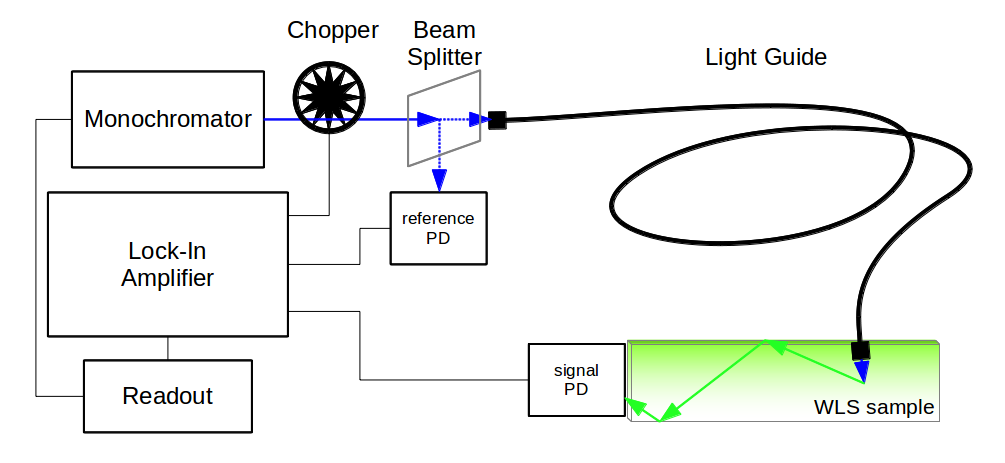
\includegraphics[width=0.7\textwidth]{Blockdiagramm}
  \end{center}
  \caption[Experimental setup]{Experimental setup for measuring the
   wavelength-dependent capture efficiency of the WLS samples.}
  \label{fig:lab_setup}
\end{figure}

A fixed setup (see Fig.~\ref{fig:lab_setup}) has been installed, which is
specifically designed to allow for the quick and easy testing of different
samples with wavelength-shifting (WLS) properties. As input radiation, the
monochromated light of a xenon arc lamp is used, which allows for scanning
wavelengths down to 200\,nm. After passing through an optical chopper, the
incident beam is split, with one beam used for monitoring the intensity of the
incoming light with a reference photo diode. The other beam is coupled to a
UV-transmitting light guide which then irradiates the sample.

The WLS sample is fixed in a mount that permits an easy exchange of samples of
different size. Therefore also the irradiating end of the light guide is
installed in a way that its position can be varied so that---apart from
accounting for different sample sizes---one is able to vary the distance between
light incidence and readout. This setup provides a handle on determining the
absorption length at the emitted wavelength.

The WLS read-out is done via a second photo diode identical to the reference
diode that is coupled to the WLS by an index-matching gel. Its output current,
as well as the one of the reference diode, is measured with a lock-in
amplifier. Using the photo diode calibration curve (response function),
along with the WLS emission spectra (Fig.~\ref{fig:capture_eff}),
the measured current is transformed into a photon flux.

For a typical measurement, the input wavelength is tuned with a resolution of
5\,nm or less in the relevant regime. At each input wavelength, the current
wavelength and the output from both diodes are stored. From this, the capture
efficiency of the WLS sample is calculated as described in
App.~\ref{app:CE_calculation}. Note that this capture efficiency includes
not only the light conversion and propagation efficiency, but also reflection
effects at the surface occurring in the measurement. The results are hence
somewhat dependant on the geometry of the WLS that is probed. Yet as the samples
match the cylindrical shape of the intended final sensor geometry, those losses
will also be present in the fully assembled module.


\section*{\refstepcounter{section}\label{app:CE_calculation}\thesection\enskip
Calculating the WLS Capture Efficiency}

The quantity that is to be extracted from the measurements is the wavelength
dependent capture efficiency of a given WLS sample, $CE(\lambda)$.

In the data recorded are only the photo currents of signal and reference diode,
$I_\mathrm{sig}(\lambda)$ and $I_\mathrm{ref}(\lambda)$, respectively. As
additional input we need a calibration measurement, which is a normal
wavelength scan without any sample installed so that the full output of the
light guide is recorded. From this we get the output fraction
\begin{equation}
 F(\lambda) =
\frac{I_\mathrm{sig,\,cal}(\lambda)}{I_\mathrm{ref,\,cal}(\lambda)} \quad .
\end{equation}

Furthermore, the response function
\begin{equation}
 R(\lambda) = I_\mathrm{out}/P_\mathrm{in}
\end{equation}
of the signal diode, which can be taken from the data sheet \cite{PD_datasheet},
has to be known and the (normalized) emission spectrum of the WLS
$S_\mathrm{WLS}(\lambda)$ needs to be measured. The finite width of the
monochromator spectrum ($\mathrm{FWHM} < 3$\,nm) is neglected.

To determine the capture efficiency, the number of photons detected when coming
out of the sample has to be divided by the number of photons radiated into the
sample. The incoming photon flux is calculated via the power emitted from the
light guide:
\begin{equation}
 P_\mathrm{in} = I_\mathrm{ref}\cdot F / R
\end{equation}
Then the photon rate is then given by
\begin{equation}
 \dot{N}_{\gamma,\,\mathrm{in}} = P_\mathrm{in} / {\textstyle
\frac{hc}{\lambda}} \quad .
\end{equation}

When calculating the detected photon rate one has to take into account that the
emitted spectrum is not monochromatic, hence one needs to average over the
relevant wavelength regime:
\begin{equation}
 \dot{N}_{\gamma,\,\mathrm{out}} = I_\mathrm{sig} / \langle R \cdot
E_\gamma\rangle \quad ,
\end{equation}
where
\begin{equation}
 \langle R \cdot E_\gamma \rangle = \int S_\mathrm{WLS}(\lambda) \, R(\lambda)
\, {\textstyle \frac{hc}{\lambda}} \,
\mathrm{d}\lambda \quad .
\end{equation}

The capture efficiency is finally given by
\begin{equation}
 CE(\lambda)=\frac{\dot{N}_{\gamma,\,\mathrm{out}}(\lambda)}{\dot{N}_{\gamma,\,
\mathrm{in}}(\lambda)}\cdot\Omega \quad ,
\end{equation}
where $\Omega$ is a factor accounting for the fact that the readout area in this
setup is smaller than it will be in a real application. Its value is given by
\begin{equation}
 \Omega = \frac{\mathrm{WLS\ front\ area}}{\mathrm{photo\ diode\ area}} \cdot 2
 \quad,
 \label{eqn:readout-area-factor}
\end{equation}
assuming that ultimately the WLS will be read over the full front area on both
ends.

\section*{\refstepcounter{section}\label{app:WOM_transmission}\thesection\enskip
Transmission into the WOM}

For light inciding into the WOM, its effective area $A_{\rm eff}$ is to be
calculated given the the WOM length $L$ (without end caps) and radius $R$. For
simplicity, we will first handle the case of frontal illumination and then
extend the result for arbitrary angles.

For the incoming light, the WOM has a rectangular cross-section of
\begin{equation}
 A_{\rm tot} = 2 R L \quad .
\end{equation}
The effective area is then given by
\begin{equation}
 A_{\rm eff} = \int_0^L {\rm d}l \cdot 2\int_0^R {\rm d}r\, T(r) = A_{\rm tot}
\cdot \varepsilon_\Omega
\end{equation}
with
\begin{equation}
 \varepsilon_\Omega = \frac{1}{R} \int_0^R {\rm d}r\, T(r) =
\int_0^{\frac{\pi}{2}} \cos\vartheta \, {\rm d}\vartheta\,
T(\vartheta), \quad \sin\vartheta = r/R
 \label{eqn:int-over-theta}
\end{equation}
and $T$ being the transmission through two consecutive optical surfaces
according to Fresnel's formulae. Since the transmission formulae are given as
functions of the angle of incidence $\theta$, it is convenient to transform
the integral in (\ref{eqn:int-over-theta}) to depend on this angle (for an
illustration see Fig.~\ref{fig:angle-of-incidence-theta}). 
Assuming the permeability is $\mu=1$, Fresnel's formulae for the transmission of
light polarised parallel and perpendicular to the optical surface read
\cite{Jackson}:
\begin{eqnarray}
 T_\parallel = 1-\left(
\frac{n_t\cos\vartheta_i-n_i\cos\vartheta_t}{
n_t\cos\vartheta_i+n_i\cos\vartheta_t}\right)^2 \\
 T_\perp = 1-\left(
\frac{n_i\cos\vartheta_i-n_t\cos\vartheta_t}{
n_i\cos\vartheta_i+n_t\cos\vartheta_t}\right)^2
\end{eqnarray}
and accordingly for unpolarised light:
\begin{equation}
 T_{\rm mean}(\theta_i,\,n_i,\,n_t) =
  \left(T_\parallel(\theta_i,\,n_i,\,n_t)
      + T_\perp(\theta_i,\,n_i,\,n_t)\right)/2 \quad .
\end{equation}
The angle of the refracted photon $\theta_t$ is given by Snell's law:
\begin{equation}
 \theta_t(\theta_i,\,n_i,\,n_t) = \arcsin\left(n_i/n_t\sin\theta_i\right)\quad.
\end{equation}

\begin{figure}
 \centering
 \subfloat[][]{
   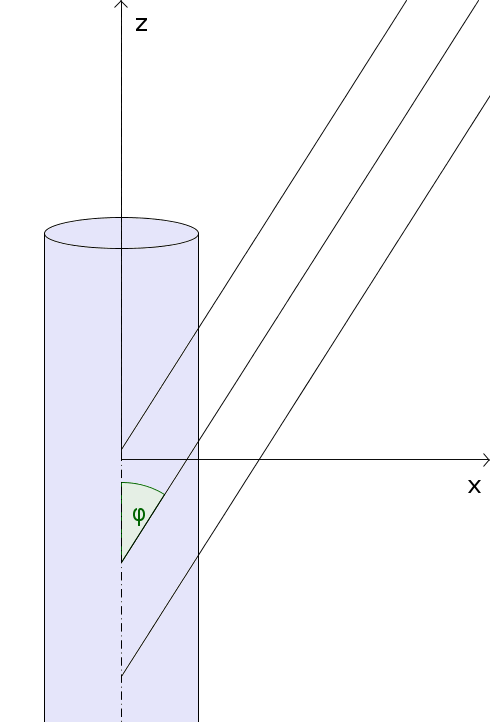
\includegraphics[height=0.3\textwidth]{phi}
   \label{fig:angle-of-incidence-phi}
 }
 \subfloat[][]{
   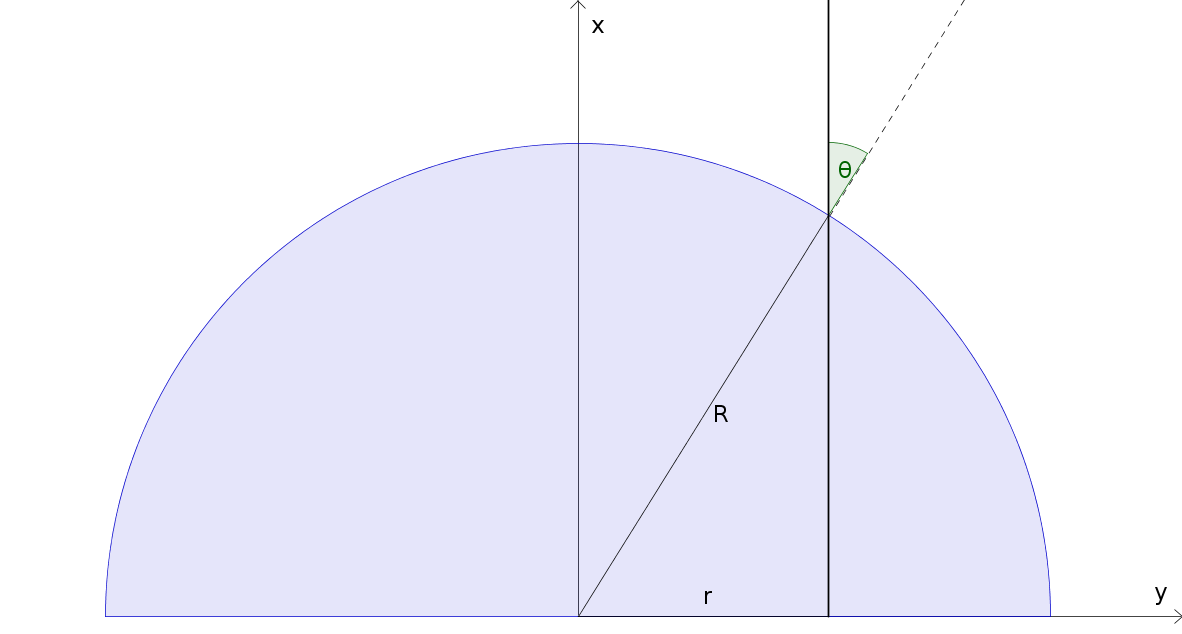
\includegraphics[height=0.3\textwidth]{theta}
   \label{fig:angle-of-incidence-theta}
 }
\caption{Definition of the angle of incidence on the WOM $\varphi$ and the
surface normal $\theta$.}
\end{figure}

The combined transmission of two surfaces with a transition from medium 1 via
medium 2 to medium 3, with refractive indices $n_1$, $n_2$, $n_3$, can be
written as the product of two transmissions of a single surface where the angle
of incidence on the second surface is given by the refraction at the first one:
\begin{equation}
 T(\vartheta,\,n_1,\,n_2,\,n_3) = T_{\rm mean}(\vartheta,\,n_1,\,n_2)\cdot
  T_{\rm mean}(\vartheta_t(\vartheta,\,n_1,\,n_2),\,n_2,\,n_3) \quad .
\end{equation}
Putting this into (\ref{eqn:int-over-theta}), the integral can be solved
numerically.

If now the incident light has an angle $\varphi\neq\pi/2$ with the WOM axis (see
Fig.~\ref{fig:angle-of-incidence-phi}),
the calculation has to be adjusted. If we choose the coordinates in a way that
the WOM axis coincides with the $z$ axis and the $x$-$z$-plane is defined by the
incident light $\hat{i}$, $\theta$ is still embedded in the $x$-$y$-plane,
but no longer equal to the angle between incident light and the surface normal
$\hat{n}$ of the WOM. The latter, however, which we will call $\alpha$, is
needed for the Fresnel transmission. It is determined by
\begin{equation}
 \cos\alpha = \hat{i}\cdot\hat{n} =
 \begin{pmatrix} \sin\varphi \\ 0 \\ \cos\varphi \end{pmatrix} \cdot
  \begin{pmatrix} \cos\vartheta \\ \sin\vartheta \\ 0 \end{pmatrix} =
 \sin\varphi\,\cos\vartheta\quad .
\end{equation}

Additionally one has to account for the fact that for light inciding at an angle
$\varphi$ the length $L$ of the WOM is jolted by a factor $\sin\varphi$.
Including all this in (\ref{eqn:int-over-theta}) one ends up with
\begin{equation}
 \varepsilon_\Omega(\varphi) = \sin\varphi \int_0^{\frac{\pi}{2}} \cos\vartheta
\, {\rm d}\vartheta\,
T\left(\alpha(\vartheta,\,\varphi)\right)\quad .
\end{equation}
The full transmission efficiency $\varepsilon_\Omega$ is plotted as a
function of $\cos\varphi$ in Fig.~\ref{fig:angular_eff}.